\section{Dynamic Analysis}

\subsection{Narrative}

We hypothesized that the book would make more sense when structured chronologically. As shown by figure~\ref{component-sizes}-A, while there are at most $12$ disconnected plot-lines in the original book order, there were as many as 19 disconnected plot-lines in the first quarter of the chronologically ordered book. It is quite a challenge to keep track of $12$ unrelated plot lines; the idea of keeping track of $19$ in Wallace's convoluted text is boggling. This makes it clear that the events in the book that occur out of chronological order provide context, and function as expositions that stitch together disparate components of the character network. On the other hand, those sections that appear chronologically provide \infinitejest's narrative structure, and move the plot of the novel forward.

Figure~\ref{component-sizes}-B shows that in both the booktime and the chronological orderings, the growth of the size of the largest component begins to slow around section 75, mirroring the point in figure~\ref{component-sizes}-A where the number of components takes a steep decline, indicating that at this point in the novel, most of the important characters have been introduced, and most of the plot lines have entered the story proper.

\begin{figure}[ht!]
    \centering
    \begin{subfigure}{0.4\textwidth}
        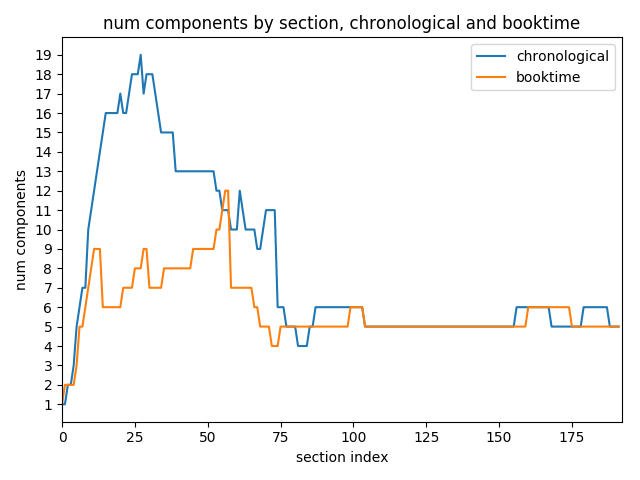
\includegraphics[width=1.\textwidth]{images/dynamics-num-components.png}
        \caption{Number of components as a function of section}
    \end{subfigure}
    \begin{subfigure}{0.4\textwidth}
        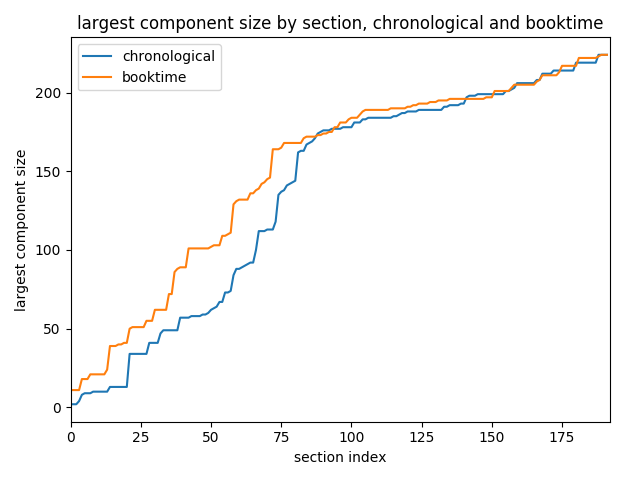
\includegraphics[width=1.\textwidth]{images/dynamics-largest-components.png}
        \caption{Largest component size as a function of section}
    \end{subfigure}
    \caption{Number of components and largest component size as a function of section}
    \label{component-sizes}
\end{figure}

\subsection{Sparsification vs Densification}

We explored whether the growth of the story's network displayed tendencies of sparsification (like an Erdos-Reyni random network, where relatively few edges are added for each new node) or of densification (where new nodes tend to add edges that complete triads).

Figure \ref{sparsification-densification}-B shows that in both the chronological and booktime orderings the mean geodesic path length increases until around $\frac{2}{3}$'s of all nodes have been added, at which point, in both orderings, the mean geodesics path lengths decrease. I.E., both orderings create a network that first sparsifies and later densifies. It is worth noting that the mean geodesic path length in the chronological ordering grows faster and achieves a higher maximum value than what is found in the booktime ordering, displaying behavior more similar to a random network than the booktime ordering. This supports the idea that the chronological ordering creates more narrative fragmentation than the booktime ordering.

Figure~\ref{sparsification-densification}-A supports the idea of sparsification followed by densification, following the same timeline as figure~\ref{sparsification-densification}-B where new nodes tend not to increase the mean degree until, again, around $\frac{2}{3}$'s of all nodes have been added, at which point new nodes tend to increase the mean degree.

\begin{figure}[ht]
    \centering
    \begin{subfigure}{0.4\textwidth}
        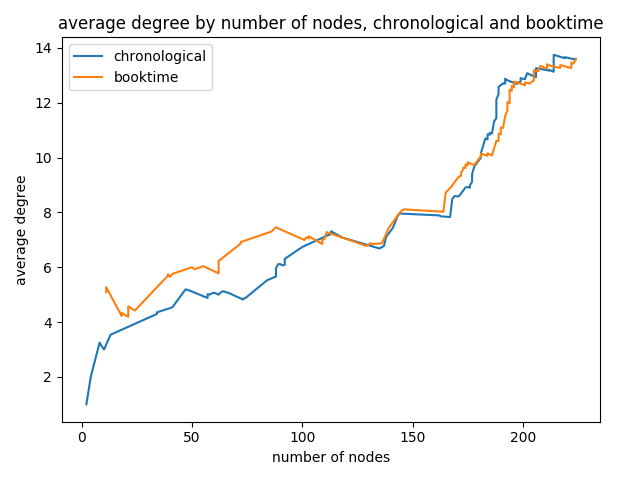
\includegraphics[width=1.\textwidth]{images/n_vs_avg_degree-weighted_False.png}
        \caption{Average unweighted degree in the largest component as a function of nodes}
    \end{subfigure}
    \begin{subfigure}{0.4\textwidth}
        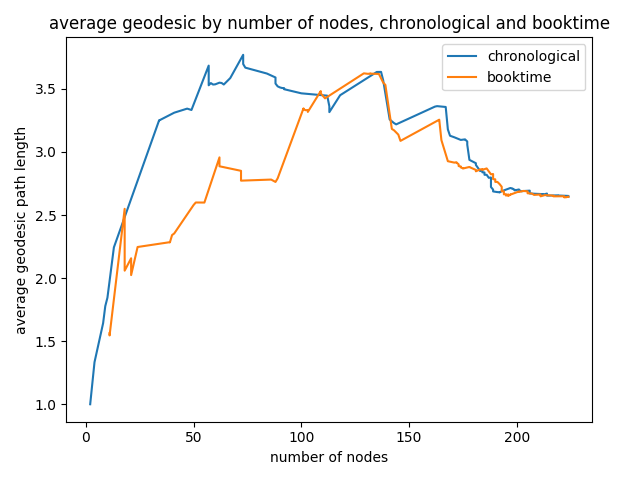
\includegraphics[width=1.\textwidth]{images/n_vs_geodesic-weighted_False.png}
        \caption{Mean geodesic path length in the largest component as a function of nodes}
    \end{subfigure}
    \caption{Node number's effect on average unweighted degree and mean geodesic path length in the largest component}
    \label{sparsification-densification}
\end{figure}

